\documentclass[10pt,spanish]{article}
\usepackage[a4paper,
top=2cm,
bottom=2cm,
includefoot,
left=3cm,
right=2cm,
footskip=1cm]{geometry}
\usepackage{url}
\IfFileExists{lmodern.sty}{\usepackage{lmodern}}{}
\usepackage{graphicx}
\usepackage{mathpazo}
\usepackage{amsmath}
\usepackage{mathptmx}
\usepackage[utf8]{inputenc}
\usepackage[T1]{fontenc}
\usepackage{color}
\usepackage[hidelinks]{hyperref}

\begin{document}

\title{Cómo Emitir una Moneda Digital del Banco Central*}
\author{David Chaum\footnote{david@chaum.com} \\
  xx Network \and
  Christian Grothoff\footnote{christian.grothoff@bfh.ch} \\
  Universidad de Ciencias Aplicadas de Berna y Proyecto GNU \and
  Thomas Moser\footnote{thomas.moser@snb.ch}\\
  Banco Nacional de Suiza}
\date{Primera versión: mayo 2020}
\maketitle

\renewcommand{\abstractname}{Resumen}
\renewcommand{\refname}{Referencias}

\begin{abstract}% [Resumen]
Con la aparición de Bitcoin y monedas estables propuestas recientemente
por grandes empresas tecnológicas como Diem (antes Libra), los bancos
centrales se enfrentan a la creciente competencia de particulares que
ofrecen su propia alternativa digital al dinero en efectivo. No
abordamos la cuestión normativa de si un un banco central debería o no
emitir una moneda digital del banco central (Central Bank Digital
Currency -- CBDC). Contribuimos en cambio al actual debate de
investigación mostrando de qué manera un banco central podría hacerlo si
así lo deseara. Proponemos un sistema basado en tokens sin tecnología de
libro mayor distribuido, y mostramos que el efectivo electrónico ya
implementado solo mediante software se puede mejorar para preservar la
privacidad en las transacciones, cumplir con los requisitos
reglamentarios de modo convincente y ofrecer un nivel de protección de
resistencia cuántica contra los riesgos sistémicos que amenazan la
privacidad. Ni la política monetaria ni la estabilidad financiera se
verían materialmente afectadas porque una CBDC con este diseño
replicaría el efectivo físico en lugar de los depósitos bancarios. \\
JEL: E42, E51, E52, E58, G2
\\
Keywords: Monedas digitales, banco central, CBDC, firmas ciegas, monedas
estables
\end{abstract}
\vspace{20pt}
\vspace{20pt}


\section*{Agradecimientos}
Agradecemos a Michael Barczay, Roman Baumann, Morten Bech, Nicolas Cuche,
Florian Dold, Andreas Fuster, Stefan Kügel, Benjamin Müller, Dirk Niepelt,
Oliver Sigrist, Richard Stallman, Andreas Wehrli, y tres colaboradores
anónimos por sus comentarios y sugerencias. Las ideas, opiniones,
investigaciones y conclusiones o recomendaciones expresadas en este
documento pertenecen estrictamente a los autores. No reflejan
necesariamente los puntos de vista del Banco Nacional de Suiza (BNS). El
BNS no asume ninguna responsabilidad por errores u omisiones ni por la
exactitud de la información contenida en este documento.

Traducción: Javier Sepulveda y Dora Scilipoti (verano 2021)


\newpage
\hypertarget{introducciuxf3n}{%
\section{Introducción}
\label{1.-introducciuxf3n}}

Desde la aparición de los ordenadores personales en los años ochenta, y
especialmente desde que en 1991 la National Science Foundation quitara
las restricciones al uso de Internet para propósitos comerciales, se ha
buscado crear dinero digital para realizar pagos en línea. La primera
propuesta la realizó Chaum en 1983. A pesar de que tales métodos fueron
implementados, no prosperaron. Fueron en cambio los sistemas con tarjeta
de crédito los que se convirtieron en el método dominante para pagos en
línea. La propuesta de Nakamoto en 2008 para un sistema P2P de dinero
digital y el posterior lanzamiento exitoso de Bitcoin desataron una
nueva era de investigación sobre el tema y desarrollo de dinero digital.
CoinMarketCap enumera más de 5.000 criptomonedas. Recientemente los
bancos centrales han empezado a considerar, o al menos estudiar, la
emisión de monedas digitales (véase Auer et. al. 2020, Boar et al. 2020,
Kiff et al. 2020 y Mancini-Griffoli et al. 2018).

Actualmente los bancos centrales emiten dos tipos de dinero: (i)
reservas en forma de cuentas de liquidación en los bancos centrales para
determinados participantes del mercado financiero y (ii) moneda en forma
de billetes disponibles para el público. En consecuencia, la
bibliografía sobre la moneda digital del banco central (CBDC) distingue
entre (a) venta de CBDC al por mayor, con acceso limitado, y (b) venta
de CBDC al por menor, accesible al público (véase, p. ej. Bech y Garratt
2017). Una CBDC al por mayor sería menos disruptiva para el sistema
actual debido a que los bancos y los participantes seleccionados del
mercado financiero ya tienen acceso a dinero digital del banco en forma
de cuentas del banco central, que utilizan para liquidar pagos
interbancarios. La cuestión aquí es si la tokenización del dinero de un
banco central y la tecnología de libro mayor distribuido (Distributed
Ledger Technology - DLT) ofrecen beneficios netos en comparación con los
sistemas de liquidación bruta en tiempo real (Real-Time Gross
Settlement - RTGS). Hasta el momento, la conclusión es que no es así, al
menos cuando se trata de pagos interbancarios nacionales (véase Chapman
et al. 2017).

Una CBDC al por menor, que sería una nueva forma de dinero del banco
central a disposición del público, podría ser más disruptiva para el
sistema actual, dependiendo de su diseño. Cuanto más compita una CBDC de
este tipo con los depósitos bancarios comerciales, mayor será la amenaza
para la financiación bancaria, con un posible impacto adverso en el
crédito bancario y la actividad económica (véase Agur et al. 2019). Sin
embargo, una CBDC al por menor podría también tener beneficios (véase
Bordo y Levin 2017, Berentsen y Schär 2018, Bindseil 2020, Niepelt 2020,
Sveriges Riksbank 2020 y Bank of England 2020). Poner a disposición de
todos dinero electrónico del banco central sin riesgo de contrapartida
podría mejorar la estabilidad y la resistencia del sistema de pago al
por menor. También podría proporcionar una infraestructura de pago
neutral para promover la competencia, la eficiencia y la innovación. En
general, es probable que los costos y beneficios de una CBDC al por
menor difieran de un país a otro. Para conocer la opinión del Banco
Nacional de Suiza, que no tiene planes de emitir una CBDC al por menor,
véase Jordan (2019).

El presente documento se centra en una CBDC al por menor, pero no
abordamos la cuestión de si un banco central \emph{debería o no} emitir
una moneda CBDC. Nos centramos en cambio en el diseño potencial de una
CBCD. Recientemente ha habido un creciente interés en el diseño de
monedas CBCD (véase p. ej. Allen et al. (2020), Bank of England (2020)).
El diseño que proponemos difiere significativamente de otras propuestas.
Nuestro sistema se basa en la tecnología eCash descrita por Chaum (1983)
y Chaum et al. (1990), mejorándola. En particular, proponemos un sistema
para CBCD basado en tokens y solo mediante software, sin blockchain para
la DLT. La DLT es un diseño interesante en ausencia de un actor
principal o si las entidades que interactúan no concuerdan en nombrar un
actor central de confianza. Sin embargo, este no es el caso de una CBCD
al por menor emitida por un \emph{banco central}. Distribuir el libro
mayor del banco central con una blockchain solo aumenta los costes de
transacción, no proporciona beneficios tangibles en una implementación
por parte de un banco central. Utilizar la DLT para emitir dinero
digital puede ser útil si no hay un banco central para empezar (p. ej.
el proyecto Sovereign de las Islas Marshall) o si la intención explícita
es prescindir de un banco central (p. ej. Bitcoin).\footnote{Puede haber
buenos casos de uso para la DLT en el caso de infraestructura de
mercado financiero, tal como los intercambios digitales, donde surge la
cuestión de como obtener dinero del banco central en la DLT a efectos de
liquidación. Sin embargo en esas situaciones, los beneficios potenciales
de la DLT, por ejemplo menos costes o reconciliación automática, no surgen
de una emisión descentralizada del dinero del banco central.}

La CBCD basada en tokens que se propone aquí permite también la
preservación de una cualidad clave del dinero físico: la privacidad en
la transacción. Usualmente se argumenta que las protecciones
criptográficas para la privacidad exigen tantos recursos computacionales
que su utilización en dispositivos móviles no es factible (véase Allen
et al. 2020). Si bien esto puede ser cierto en el contexto de la DLT,
donde la rastreabilidad pública de las transacciones es necesaria para
prevenir el doble gasto (Narayanan et al. 2016), no es cierto para el
protocolo de firma ciega de tipo Chaum con un banco central que se
propone en el presente documento. Nuestra CBDC, basada en firmas ciegas
y arquitectura de dos niveles, garantiza una perfecta privacidad de
resistencia cuántica en las transacciones, al mismo tiempo que
proporciona protecciones sociales tales como impedir el lavado de dinero
(Anti-Money Laundering - AML) y financiar la lucha contra el terrorismo
(Counter Terrorism Financing -- CFT), protecciones que de hecho tienen
mayor fuerza que con los billetes.

La privacidad en las transacciones es importante por tres razones.
Primero, porque protege a los usuarios frente al escrutinio y el abuso
de vigilancia gubernamental. Los programas de vigilancia masiva son
problemáticos incluso si las personas creen que no tienen nada que
esconder, simplemente por la posibilidad de error y abuso,
particularmente si los programas carecen de transparencia e
imputabilidad (véase Solove 2011). Segundo, porque la privacidad en las
transacciones protege a los usuarios frente a la explotación de datos por parte
de los proveedores de servicios de pago.
Tercero, porque protege a los usuarios frente a la contraparte en la
transacción, descartando la posibilidad de un posterior comportamiento
oportunista, o frente a riesgos de seguridad debido a fallos o
negligencia en la protección de los datos del cliente (véase Kahn et al.
2005).

Este documento está estructurado como sigue: en la sección 2 explicamos
la diferencia entre el dinero del banco central y otro dinero. En la
sección 3 analizamos los diseños de CBDC comunes y simplistas, antes
de proponer nuestro diseño en la sección 4. Luego comentamos
consideraciones políticas y normativas (5) y trabajos relacionados (6);
en fin, concluimos (7).

\hypertarget{quuxe9-es-el-dinero-del-banco-central}{%
\section{¿Qué es el dinero del banco central?} \label{2.-quuxe9-es-el-dinero-del-banco-central}}

El dinero es un activo que puede ser usado para comprar bienes y
servicios. Para ser considerado dinero, este activo debe ser aceptado
por otras entidades distintas del emisor. Este es el motivo por el que
los vales, por ejemplo, no se consideran dinero. El dinero genuino tiene
que ser aceptado \emph{comúnmente} como medio de intercambio. Si bien el
dinero tiene otras funciones, por ejemplo como unidad de cuenta y
depósito de valor, la característica que lo distingue es su función como
medio de intercambio. Normalmente, la unidad de cuenta (p. ej. cómo se
cotizan los precios y cómo se registran las deudas) coincide con el
medio de intercambio por razones de conveniencia. La separación puede
ocurrir, sin embargo, si el valor del medio de intercambio carece de
estabilidad en relación a los bienes y servicios
comercializados.\footnote{Esto puede ocurrir espontáneamente en un entorno
de alta-inflación, p. ej. cuando los precios se fijan en USD pero los pagos
se realizan en divisa local. Lo mismo es ciertopara los pagos en Bitcoin,
donde los precios usualmente se fijan en USA u otras divisas locales debido a
la alta volatilidad de Bitcoin. Una eparación también puede ocurrir por el
diseño, p. ej. en la Unidad de Fomento (UF) de Chile o la Special Drawing Right
(SDR) del fondo monetario internacional (IMF). Sin embargo, también entonces el
propósito es tener una unidad de cuenta más estable.} El dinero debe también ser
un depósito de valor para poder actuar como medio de intercambio, porque
debe preservar su poder de compra desde el momento en que se recibe
hasta el momento en que se gasta. Sin embargo, varios otros activos
sirven como depósito de valor, como por ejemplo acciones, bonos, metales
preciosos e inmuebles. Por tanto, la característica como depósito de
valor no es distintiva del dinero.

En la economía moderna, el público usa dos tipos diferentes de dinero:
(a) dinero estatal y (b) dinero privado. El dinero estatal lo emite
típicamente un banco central, que actúa como agente del Estado. El
dinero del banco central está disponible para determinadas instituciones
financieras en forma de depósitos en el banco central (reservas) y para
el público en forma de moneda (billetes y monedas), también llamado
``efectivo''. En una economía moderna con dinero fiduciario, tal dinero
no tiene valor intrínseco. Legalmente es una obligación del banco
central, aunque no es canjeable.

En la mayoría de los países, el dinero del banco central se define como
moneda de curso legal, lo cual significa que debe ser aceptado como pago
de una deuda monetaria, incluyendo impuestos y multas legales. Si bien
esto garantiza que el dinero del banco central tenga algún valor, el
estatus de moneda de curso legal es insuficiente para que el dinero del
banco central mantenga un valor estable. Más bien, es la política
monetaria de los bancos centrales la que mantiene el valor del dinero.
Mantener la estabilidad de los precios, es decir, un valor estable del
dinero en relación con el valor de los bienes y servicios
comercializados, es una de las principales responsabilidades de los
bancos centrales.

En una economía moderna, la mayoría de los pagos se hacen con dinero
privado emitido por bancos comerciales. Tal dinero se compone de
depósitos a la vista que la gente tiene en los bancos comerciales. A
estos depósitos bancarios se puede acceder con cheques, tarjetas de
débito, tarjetas de crédito, u otros medios para transferir dinero. Son
una obligación del respectivo banco comercial. Una característica
fundamental de los depósitos bancarios es que los bancos comerciales
garantizan la convertibilidad, bajo demanda, en dinero del banco central
a un precio fijo, es decir, a la par. Los depositantes pueden retirar
sus fondos en efectivo o transferirlos a una tasa fija de 1:1. Los
bancos comerciales mantienen estable el valor de su dinero vinculándolo
al dinero del banco central.

No obstante, en un sistema de reserva fraccionado, un banco comercial
-- incluso siendo solvente -- puede no contar con la liquidez necesaria
para cumplir su promesa de convertir los depósitos bancarios en dinero
del banco central (p. ej. en caso de una caída bancaria) de manera tal
que los clientes no puedan retirar su dinero. Un banco también puede
llegar a ser insolvente e ir a la bancarrota, y como resultado los
clientes pueden perder su dinero. Así, los bancos comerciales están
regulados para mitigar estos riesgos.

Una diferencia significativa entre el dinero de un banco central y el
dinero emitido privadamente por un banco comercial es, por lo tanto, que
este último conlleva un riesgo para la contraparte. Un banco central
puede siempre cumplir con sus obligaciones usando su propio dinero no
reembolsable. El dinero del banco central es el único activo monetario
de una economía nacional sin riesgo crediticio o de liquidez. Por lo
tanto, es el activo que típicamente se prefiere para los pagos en las
infraestructuras del mercado financiero (véase p. ej. CPMI-IOSCO
\emph{Principles for Financial Market Infrastructures}, 2012). Otra
diferencia es que el dinero del banco central afianza el sistema
monetario nacional al proporcionar una referencia de valor con la que el
dinero de los bancos comerciales mantiene una convertibilidad a la par.

Aparte de los bancos comerciales, otra entidades privadas ocasionalmente
intentan emitir dinero, las criptomonedas son solo el intento más
reciente. Pero a diferencia de los depósitos bancarios, tal dinero no es
comúnmente aceptado como medio de intercambio. Esto también sucede con
Bitcoin, la criptomoneda más aceptada. Un impedimento a su utilidad como
medio de intercambio es la alta volatilidad de su valor. Una respuesta
reciente a este problema fue la aparición de las llamadas monedas
estables. Las monedas estables generalmente intentan estabilizar su
valor en una de las dos maneras siguientes: o bien imitando a los bancos
centrales (monedas estables algorítmicas) o bien imitando a los bancos
comerciales o a los medios de inversión (monedas estables con respaldo
de activos).\footnote{Para más detalles sobre la taxonomia y descripción
de las monedas stables véase Bullman et al. (2019).}

Las ``monedas estables algorítmicas'' dependen de algoritmos para
regular su suministro. En otras palabras, intentan alcanzar la
estabilidad de su precio con sus propias ``políticas monetarias
algorítmicas''. Hay ejemplos de tales monedas estables (p. ej. Nubits),
pero hasta ahora ninguna ha estabilizado su valor por largo tiempo.

Las monedas estables ``respaldadas con activos'' difieren en función del
tipo de activos que usan y de los derechos legales que adquieren los
titulares de monedas estables. Los tipos de activos que típicamente se
usan son: dinero (reservas del banco central, billetes o depósitos en
bancos comerciales), productos básicos (p. ej. oro), valores y a veces
otras criptomonedas. Cuán bien tal esquema estabilice el valor de las
monedas en relación al activo o los activos subyacentes depende de
manera crucial de los derechos legales que adquieran los titulares de
las monedas estables. Si una moneda estable es canjeable a un precio
fijo (p. ej. 1 moneda = 1 USD, o 1 moneda = 1 onza de oro), tal
estabilidad teóricamente se conseguirá.\footnote{Si también estabilice o
no el valor de las monedas estables en relación con los bienes y
servicios negociados depende de la estabilidad del valor del respectivo
activo en relación con el valor de los bienes y servicios.} Lo que el esquema
esencialmente hace es replicar a los bancos comerciales garantizando la
convertibilidad al activo subyacente a la vista. Sin embargo, a
diferencia de los depósitos bancarios, que típicamente están solo
parcialmente respaldados por las reservas monetarias del banco central,
las monedas estables generalmente están respaldadas completamente por
las reservas del activo subyacente para evitar el riesgo de liquidez,
principalmente porque carecen de beneficios públicos tales como el
soporte de seguros de depósito y prestamistas de última instancia, que
se aplican en cambio a los bancos regulados.

Las monedas estables respaldadas con dinero se llaman también monedas
estables fiduciarias. Sin embargo, mantener el 100\% de garantía en
dinero (billetes o depósitos bancarios) no es muy rentable. En
consecuencia, los proveedores de monedas estables tienen un incentivo
para economizar su tenencia de activos y trasladarse hacia un sistema de
reserva fraccionado, tal como lo hicieron los bancos comerciales.\footnote
{La incertidumbre sobre si un moneda estable está
totalmente garantizada puede ser una de las razones por las que una
moneda stable puede negociarse por debajo de la par en el mercado
secundario (véase Lyons y Ganesh Viswanath-Natraj, 2020). Este fue
también historícamente el caso con los billetes cuando eran emitidos
por los bancos comerciales. Tales billetes solían negociarse con
diversos descuentos en el mercado secundario antes de que la emisión
de billetes fuera nacionalizada y transferida al monopolio de los
bancos centrales.} Esto implica que reducen su tenencia de activos de
bajo rendimiento al mínimo que se considere necesario para satisfacer el
requisito de convertibilidad. Añadiendo en cambio activos líquidos de
alto rendimiento tales como bonos del Estado. Esto mejora la
rentabilidad pero también incrementa el nivel de riesgo.

Sin embargo, incluso si una moneda estable está garantizada al 100\% por
un depósito en un banco comercial, sigue expuesta a los riesgos de
crédito y liquidez del banco subyacente. Este riesgo se puede eliminar
si los depósitos se mantienen en el banco central para que la moneda
estable esté respaldada por las reservas del banco central. Tales
monedas estables han sido llamadas ``CBDC sintéticas'' (Adrian y
Mancini-Griffoli 2019). Es importante señalar, sin embargo, que tales
monedas estables no son dinero del banco central y por lo tanto no son
CBDC, ya que no constituyen obligaciones del banco central y, por lo
tanto, siguen expuestas al riesgo de contraparte, es decir, el riesgo de
que el emisor de la moneda estable se declare en quiebra.

Si una moneda estable no es canjeable a un precio fijo, su estabilidad
no está garantizada por el activo subyacente. Si la moneda estable a
pesar de esto representa una participación en la propiedad del activo
subyacente, el esquema se asemeja a un fondo de inversión fijo o a un
fondo cotizado en bolsa (Exchange-Traded Fund - ETF), y se aplican los
correspondientes riesgos. El valor de la moneda dependerá del valor neto
de los activos del fondo, pero su valor real puede desviarse. Si hay
participantes autorizados que puedan crear y canjear monedas estables y
así actuar como arbitristas, como en el caso de los ETF y como estaba
previsto para Diem (Asociación Libra 2020), es probable que la
desviación sea mínima.

En general, las monedas estables tiene una mayor probabilidad de llegar
a convertirse en dinero que las criptomonedas, especialmente si se
regulan adecuadamente. Sin embargo, la disponibilidad de CBDC limitaría
significativamente su utilidad.

\hypertarget{diseuxf1os-simplistas-de-cbdc}{%
\section{Diseños simplistas de CBDC} \label{3.-diseuxf1os-simplistas-de-cbdc}}

Como se ha señalado, una CBDC sería una obligación del banco central.
Dos posibles diseños que se analizan en la literatura son: (a) una CBDC
basada en cuentas y (b) una CBDC basada en tokens (o basada en valor).
Estos diseños corresponden a los dos tipos existentes de dinero de un
banco central y sus correspondientes sistemas de pago (Kahn y Roberds
2008): las reservas de un banco central (en un sistema basado en
cuentas) y billetes (en un sistema basado en tokens). Un pago se produce
si un activo monetario se transfiere de un pagador a un beneficiario. En
un sistema basado en cuentas, una transferencia se produce cobrándole a
la cuenta del pagador y transfiriendo el crédito a la cuenta del
beneficiario. En un sistema basado en tokens, la transferencia se
produce transfiriendo el valor en sí o el token, es decir, un objeto que
representa el activo monetario. El mejor ejemplo de un token es el
efectivo -- monedas o billetes. Pagar con efectivo significa entregar
una moneda o un billete. No es necesario registrar la transferencia, la
posesión del token es suficiente. Por lo tanto, las partes no están
obligadas a revelar sus identidades en ningún momento durante la
transacción, ambas pueden permanecer anónimas. De todas maneras, el
beneficiario tiene que poder verificar la autenticidad del token. Esta
es la razón por la que los bancos centrales invierten mucho en elementos
de seguridad para los billetes.

Ha habido sugerencias de que la distinción entre los sistemas basados en
cuentas y los sistemas basados en tokens no es aplicable a las monedas
digitales (Garratt et al. 2020). Nosotros tenemos una opinión diferente
porque creemos que hay una diferencia significativa. La distinción
fundamental es la información contenida en el activo. En un sistema
basado en cuentas, los activos (las cuentas) se asocian con los
historiales de las transacciones, que incluyen todas las operaciones de
crédito y débito de las cuentas. En un sistema basado en tokens, los
activos (tokens) incluyen información acerca de su valor y de la entidad
que emitió el token. Por tanto, la única posibilidad de lograr la
propiedad de privacidad de la transacción como la que se obtiene con el
dinero efectivo reside en los sistemas basados en tokens.\footnote
{Si bien el término "Bitcoin" sugiere el uso de tokens, Bitcoin es un
sistema basado en cuentas. La única diferencia entre un sistema
tradicional basado en cuentas y una blockchain es que las cuentas no
se guardan en una base de datos central, sino en una base de datos
descentralizada del tipo "solo por anexión".}

\hypertarget{cbdc-basada-en-cuentas}{%
\subsection{CBDC basada en cuentas}\label{cbdc-basada-en-cuentas}}

La forma más simple de lanzar una CBDC sería permitir que el público
tenga cuentas de depósito en el banco central. Esto implica que el banco
central seria responsable de llevar a cabo verificaciones para conocer a
sus clientes (Know-Your-Customer - KYC) y asegurar el cumplimiento del
AML y CFT. Esto incluiría no solo realizar el proceso inicial del KYC,
sino también autentificar a los clientes para las transacciones
bancarias, gestionar el fraude y lidiar con los falsos positivos y las
autenticaciones de los falsos negativos. Dada la limitada presencia
física de bancos centrales en la sociedad, y el hecho de que la
autenticación del ciudadano es algo que probablemente en la actualidad
los bancos no estén preparados para hacer a gran escala, cualquier CBDC
basada en cuentas requeriría que el banco central delegara estas
verificaciones. Todo el servicio y mantenimiento de tales cuentas podría
asignarse a proveedores externos (Blindseil 2020), o la legislación
podría obligar a los bancos comerciales a abrir cuentas bancarias en el
banco central para sus clientes (Berentsen y Schär 2018).

Tal CBDC basada en cuentas daría potencialmente a un banco central mucha
información. Una posible preocupación podría ser que esto permitiera a
los gobiernos realizar fácilmente vigilancia masiva e imponer sanciones
a los titulares de cuentas individuales. Su naturaleza centralizada hace
que tales intervenciones sean económicas y fáciles de aplicar contra
individuos o grupos. Incluso en las democracias, hay muchos ejemplos de
abusos de vigilancia dirigidos a críticos y opositores políticos. Se
podría argumentar que los bancos centrales independientes puedan
salvaguardar tal información del escrutinio del gobierno y el abuso
político, pero esto solo abriría una nueva vía para la presión política,
amenazando la independencia del banco central. Además, la base de datos
central sería un objetivo importante para los atacantes: incluso el
acceso de solo lectura a partes de la base de datos podría crear riesgos
significativos para las personas cuyos datos fueran expuestos.

Proveyendo cuentas bancarias al público, un banco central estaría
también en competición directa con los bancos comerciales. Esta
competición implicaría dos riesgos. Primero, podría amenazar la base de
depósitos de los bancos y, en el extremo, desintermediar el sector
bancario. Esto podría afectar de manera adversa la disponibilidad de
crédito para el sector privado y, como resultado, la actividad económica
(Agur et al. 2019). La desintermediación de los bancos también podría
conducir a la centralización del proceso de asignación de crédito dentro
del banco central, lo que afectaría negativamente la productividad y el
crecimiento económico. En segundo lugar, permitir que la gente traslade
sus depósitos al refugio seguro de un banco central podría acelerar las
caídas bancarias durante crisis financieras.

Existen sin embargo argumentos contrarios. Brunnermeier y Niepelt (2019)
argumentan que la transferencia de fondos desde un depósito hacia una
cuenta de CBDC conduciría a una sustitución automática de la
financiación de depósitos por la financiación del banco central,
simplemente haciendo explicita la garantía implícita del banco central
como prestamista de última instancia. Berentsen y Schär (2018) sostienen
que la competencia de los bancos centrales podría incluso tener un
efecto disciplinario sobre los bancos comerciales y, por lo tanto,
incrementar la estabilidad del sistema financiero, ya que los bancos
comerciales tendrían que hacer sus modelos de negocio más seguros para
evitar las caídas bancarias.

También hay propuestas para mitigar el riesgo de la desintermediación
que tienen como objetivo limitar o desincentivar el uso de CBDC como
depósito de valor. Una propuesta es limitar la cantidad de CBDC que se
puede poseer. Una segunda propuesta es aplicar una tasa de interés
ajustable a las cuentas de CBDC, de manera que la remuneración esté
siempre lo bastante por debajo de la remuneración de las cuentas de los
bancos comerciales (posiblemente incluyendo un rendimiento negativo)
para hacer que las CBDC resulten menos atractivas como depósitos de
valor (Kumhof y Noone 2018, Bindseil 2020). Además, para disuadir las
caídas bancarias, Kumhof y Noone (2018) sugieren que las CBDC no
deberían ser emitidas contra depósitos bancarios, sino solo contra
valores tales como bonos del Estado. En general, una CBDC basada en
cuentas requeriría un análisis más profundo de estas cuestiones.

\hypertarget{cbdc-basada-en-tokens-y-dependiente-del-hardware}{%
\subsection{CBDC basada en tokens y dependiente del hardware}
\label{cbdc-basada-en-tokens-y-dependiente-del-hardware}}

Un banco central podría también emitir tokens electrónicos en lugar de
cuentas. Técnicamente esto requiere de un sistema para asegurar que los
tokens electrónicos no se puedan copiar fácilmente. Las funciones
físicamente imposibles de clonar (véase Katzenbeisser et al. 2012) y las
zonas seguras en el hardware (véase Alves y Felton 2004, Pinto y Santos
2019) son dos tecnologías potenciales para la prevención de la copia
digital. Las funciones físicas imposibles de clonar, sin embargo, no se
pueden intercambiar a través de Internet (eliminando así el uso
principal de las CBDC), y anteriores funciones de seguridad en el
hardware para la prevención de copias se han visto comprometidas
repetidamente (véase p. ej. Wojtczuk y Rutkowska 2009, Johnston 2010,
Lapid and Wool 2019).

Una ventaja fundamental de las CBDC basadas en tokens sobre las basadas
en cuentas del banco central es que los sistemas basados en tokens
funcionarían sin conexión, es decir, los usuarios podrían intercambiar
tokens (peer-to-peer) sin involucrar al banco central, lo que protegería
la privacidad y la libertad de las personas. Sin embargo, la
desintermediación que se produce cuando los usuarios pueden intercambiar
tokens electrónicos sin los bancos como intermediarios que realizan los
controles KYC, AML y CFT dificultarían la limitación de los abusos por
parte de delincuentes.

Las tarjetas SIM son actualmente las candidatas más extensivamente
disponibles para un sistema de pago seguro basado en hardware, pero
estas también conllevan riesgos. La experiencia (véase p. ej. Soukup y
Muff 2007, Garcia et. al. 2008, Kasper et. al. 2010, CCC 2017) sugiere
que cualquier dispositivo económicamente producible que almacene tokens
con un valor monetario en posesión de una persona, y que permita
transacciones sin conexión -- y por tanto el robo de la información que
contiene -- será el objetivo de ataques de falsificación exitosos tan
pronto como el valor económico del ataque fuera los suficientemente
elevado. Tales ataques incluyen usuarios que atacan su propio hardware
(véase también Allen et al. 2020). Los sistemas de pago con tarjeta que
se han desplegado previamente dependen de la resistencia a la
manipulación en combinación con la detección del fraude para limitar el
impacto de una situación de peligro. Sin embargo, la detección del
fraude requiere la habilidad de identificar a los pagadores y seguir la
pista de los clientes, lo cual no es compatible con la privacidad de la
transacción.

\hypertarget{diseuxf1o-de-cbdc-basado-en-tokens-para-salvaguardar-la-privacidad}{%
\section{Diseño de CBDC basado en tokens para salvaguardar la
privacidad}
\label{4.-diseuxf1o-de-cbdc-basado-en-tokens-para-salvaguardar-la-privacidad}}

La CBDC que se propone aquí es de tipo "solo software", simplemente una
aplicación para teléfonos inteligentes que no requiere ningún hardware
adicional por parte de los usuarios. La CBDC se basa en eCash y GNU
Taler. Taler es parte del Proyecto GNU, cuyo fundador, Richard Stallman,
acuñó el término \emph{Software Libre}, actualmente denominado \emph{Software
Libre y de Código Abierto} (Free/Libre Open Source Software --
FLOSS).\footnote{Para más información sobre GNU, véase
\url{https://www.gnu.org} y Stallman (1985). GNU Taler se publica
gratuitamente bajo la Licencia Pública General Affero del Proyecto
GNU. Otros programas del Proyecto GNU populares entre los economistas
son «R» y ``GNU Regression, Econometrics and Time-series Library''
(GRETL). Un análisis de los beneficios del FLOSS en comparación con el
software privativo en el campo de la investigación puede consultarse
en Baiocchi y Distaso (2003), Yalta y Lucchetti (2008) y Yalta y Yalta
(2010). Sobre el licenciamiento de código abierto véase Lerner y
Tirole (2005).} Un programa se considera "Software Libre" si la licencia
otorga a los usuarios cuatro libertades esenciales: la libertad
de ejecutar el programa como deseen, la libertad de estudiar el programa
y modificarlo, la libertad de redistribuir copias del programa y la
libertad de distribuir copias de las versiones modificadas del programa.
El software libre no tiene por qué ser no comercial: proporcionar
soporte técnico para software es un modelo de negocio estándar para el
FLOSS.

Dado el gran número de partes interesadas involucradas en una CBDC al
por menor (el banco central, el sector financiero, comerciantes y
clientes) y la importancia crítica de la infraestructura, una CBDC al
por menor debe basarse en el FLOSS. Imponer una solución propietaria que
requiera la dependencia de un proveedor en particular sería
probablemente un obstáculo para la adopción desde el principio. Con el
FLOSS, todas las partes interesadas tienen acceso a cada detalle de la
solución y el derecho de adaptar el software a sus necesidades. Esto
conduce a una integración más fácil y una mejor interoperabilidad y
competencia entre proveedores.\footnote{Sin embargo, puede haber otros
roles para hardware privado. Por ejemplo, proteger los depósitos de
claves y ciertas funciones de auditoría, en la medida en que tal
seguridad pueda demostrarse solo como aditiva, puede ser un área donde
el hardware dedicado evaluado por solo un número limitado de expertos
podría tener ventajas.} Además, permite que el banco central cumpla
con los requisitos de transparencia y responsabilidad. Los beneficios
del FLOSS para la seguridad son también ampliamente reconocidos. La
disponibilidad del código fuente y el derecho a modificarlo facilitan la
detección de fallos y su rápida solución.\footnote{Por ejemplo, un
boletín de seguridad cibernética emitido por la Agencia de Seguridad
Nacional de EE. UU. en abril de 2020 insta a los usuarios a priorizar
el software de código abierto en la selección y el uso de servicios de
colaboración para la comunicación por Internet: ``El desarrollo de
código abierto puede proporcionar confiabilidad de que el código está
escrito para asegurar las mejores prácticas de programación y no es
probable que introduzca vulnerabilidades o debilidades que puedan
poner en riesgo a los usuarios y los datos '' (U/OO/134598-20).}

En esta nuestra arquitectura que proponemos todas las interacciones del
consumidor y el comerciante son con bancos comerciales. Sin embargo, la
creación de dinero y la base de datos las proporcionan exclusivamente el
banco central. Los bancos comerciales autentican a los clientes cuando
retiran CBDC y a los comerciantes/beneficiarios cuando reciben CBDC,
pero cuando gastan CBDC, los clientes/pagadores solo tienen que
autorizar sus transacciones y no necesitan identificarse. Esto hace que
los pagos resulten más baratos, fáciles y rápidos, y evita una fácil
interferencia con la privacidad (Dold 2019). Además, autenticar a los
clientes cuando retiran CBDC y a los comerciantes/beneficiarios cuando
reciben CBDC garantiza el cumplimiento del KYC, AML y CFT.

La CBDC que se propone en el presente documento es un auténtico
instrumento digital al portador porque cuando el usuario retira una suma
de dinero en forma de número, el número es ``cegado'' u ocultado por el
teléfono inteligente con un cifrado especial. En el sistema real, una
moneda es un par de claves pública / privada, y la clave privada solo la
conoce el propietario de la moneda.\footnote{En Bitcoin, que es un
sistema basado en cuentas, el par de claves es una cuenta, siendo la
clave pública la "dirección" de la cuenta y por tanto un tipo de
"identidad'', incluso si se trata de un pseudónimo.} La moneda deriva
su valor financiero de la firma del banco central en la clave pública de
la moneda. El banco central hace la firma con su clave privada y dispone
de múltiples pares de claves de denominación para la firma ciega de
monedas de diferentes valores. Un comerciante puede utilizar la
correspondiente "clave pública" del banco central para verificar la
firma. Sin embargo, para asegurarse de que la moneda no haya sido
copiada y ya canjeada por otro beneficiario (es decir, que no se haya
"gastado dos veces"), el comerciante debe depositar la moneda para que
el banco central pueda comparar la moneda con un archivo de monedas
canjeadas. Debido a que ni el banco comercial ni el banco central ven el
número de la moneda durante el retiro, más tarde, cuando el comerciante
deposita la moneda, se desconoce qué usuario la retiró. El cegamiento y
la privacidad resultante son los que hacen de este tipo de CBDC un
verdadero instrumento digital al portador.

En el análisis que sigue proporcionamos una introducción de alto nivel a
la tecnología y demostramos cómo se puede integrar con el sistema
bancario existente para crear una CBDC. Dold (2019) describe detalles
adicionales.

\hypertarget{componentes-fundamentales}{%
\subsection{Componentes fundamentales}\label{componentes-fundamentales}}

A continuación describimos los principales componentes del protocolo,
incluido el trasfondo matemático para una posible instanciación de las
primitivas criptográficas utilizadas, para ilustrar cómo podría
funcionar una implementación. Observamos que existen diseños matemáticos
alternativos y equivalentes para cada componente, y simplemente
presentamos los diseños seguros más sencillos de los que tenemos
conocimiento.

\emph{Firmas digitales.} La idea básica de las firmas digitales en un
esquema de firma con clave pública es que el propietario de una clave
privada es el único que puede firmar un mensaje, mientras que la clave
pública permite a cualquiera verificar la validez de la
firma.\footnote{La criptografía de clave pública fué introducida por
Diffie y Hellman (1976), y la primera implentación de firmas digitales
fué introducida por Rivest, Shamir y Adleman (1978).} El resultado de
la función de verificación es la declaración binaria "verdadero" o
"falso". Si el mensaje está firmado con la clave privada que pertenece a
la clave pública de verificación, el resultado es verdadero, de lo
contrario es falso. En nuestra propuesta, el mensaje es una "moneda" o
"billete" con un número de serie, y la firma del banco central confirma
su validez. Si bien GNU Taler usa por defecto firmas EdDSA modernas
(véase Bernstein et al. 2012), presentamos un esquema de firma
criptográfica simple basado en el bien estudiado sistema criptográfico
RSA (Rivest et al. 1978).\footnote{Para un análisis de la larga historia
del criptosistema RSA y un estudio de los ataques al criptosistema RSA,
consulte Boneh (1999).} Sin embargo, en principio se puede utilizar
cualquier esquema de firma criptográfica (DSA, ECDSA, EdDSA, RSA, etc.).

Para generar las claves RSA, el firmante elige primero dos grandes e
independientes números primos $p$ y $q$ y calcula $n = \emph{pq}$
así como la función totient de Euler
$\phi(n) = (p - 1)(q - 1)$.
Entonces, cualquier $e$ con $1 < e < \phi(n)$ y
$\gcd(e, \phi(n)) = 1$ se puede usar para
definir una clave pública $(e,n)$. La condición de que el
mayor común divisor (greatest common divisor - $\gcd$) de $e$ y
$\phi(n)$ tiene que ser 1 (p. ej., que deben ser
relativamente primos) asegura que la inversa de
$e \mod \phi(n)$ existe.
Esta inversa es la
correspondiente clave privada $d$. Dado $\phi(n)$, la clave
privada $d$ se puede calcular usando el algoritmo extendido
Euclídeo de modo que
$d \cdot e \equiv 1 \mod \phi(n)$.

Dada la clave privada $d$ y la clave pública $(e, n)$, una firma simple RSA
$s$ sobre un mensaje $m$ es
$s \equiv m^{d} \mod n$.
Para verificar la firma, se calcula
$m' \equiv s^{e} \mod n$.
Si $m'$ y $m$ coinciden, la firma es válida, lo que prueba que el
mensaje fue firmado con la clave privada que pertenece a la clave
publica de verificación (autenticación de mensaje) y que ese mensaje no
ha sido cambiado en tránsito (integridad de mensaje). En la práctica,
las firmas se colocan sobre lo hashes de los mensajes en vez de los
propios mensajes. Las funciones hash calculan el resumen de los
mensajes, que son identificadores únicos y cortos para los mensajes.
Firmar un hash corto es mucho más rápido que firmar un mensaje largo, y
la mayoría de los algoritmos de firma solo funcionan con entradas
relativamente cortas.\footnote{En el caso del criptosistema RSA el
límite de la longitud es $\log_{2}n$ bits.}

\emph{Firmas ciegas.} Usamos firmas ciegas, introducidas por Chaum
(1983), para proteger la privacidad de los compradores. Una firma ciega
se usa para crear una firma criptográfica para un mensaje sin que el
firmante conozca el contenido del mensaje que se firma. En nuestra
propuesta, esto evita que los bancos comerciales y el banco central
puedan rastrear las compras identificando a los compradores. Nuestra
propuesta funciona en principio con cualquier esquema de firma ciega,
pero la mejor solución es la variante basada en RSA descrita por Chaum
(1983).

El cegamiento lo realizan los clientes, quienes ciegan sus monedas antes
de transmitirlas al banco central para ser firmadas. Los clientes por
tanto no necesitan confiar al banco central la protección de su
privacidad. Además, el cegamiento RSA proveería de protección de la
privacidad incluso contra ataques informáticos cuánticos. El banco
central, por su parte, establece múltiples denominaciones de pares de
claves disponibles para realizar la firma ciega de monedas con
diferentes valores, y publica/provee las correspondientes claves
públicas $(e, n)$ para estos valores.

Sea $f$ el valor hash de una moneda y por tanto un identificador único
para esta moneda. El cliente que retira la moneda primero genera una
factor ciego aleatorio $b$ y calcula
$f' \equiv fb^{e} \mod n$
con la clave pública del banco central para ese valor.
La moneda cegada $f'$ se transmite luego
al banco central para ser firmada. El banco central firma $f'$ con su
clave privada $d$ calculando la firma ciega
$s' \equiv \left(f' \right)^{d} \mod n$,
añade la firma $s'$ a la moneda cegada $f'$ y devuelve el par
$(s',f')$ al cliente.
El cliente puede entonces des-cegar la firma calculando
$s \equiv s'b^{- 1} \mod n$.
Esto funciona porque
$\left( f' \right)^{d} = f^{d}b^{\text{ed}} = f^{d}b$ y, así,
multiplicar $s'$ con $b^{- 1}$ produce $f^{d}$, que es una firma RSA
válida sobre $f$ como antes:
$s^{e} \equiv f^{\text{de}} \equiv f \mod n$.

En la propuesta original de Chaum, las monedas eran solo tokens. Sin
embargo, nosotros queremos que los consumidores puedan realizar
contratos usando firmas digitales. Para lograrlo, cuando una billetera
digital retira una moneda, primero crea una clave privada aleatoria
$c$ y calcula la correspondiente clave publica $C$ de esta moneda
para crear firmas digitales con esquemas de firma criptográfica
regulares (como DSA, ECDSA, EdDSA y RSA). Entonces, se deriva $f$
usando una hash criptográfica de la clave pública $C$, que luego es
firmada en modalidad ciega por el banco central (usando un factor
aleatorio ciego actualizado para cada moneda). Ahora el cliente puede
usar $c$ para firmar compras electrónicamente, gastando así la moneda.

Como se ha señalado anteriormente, el banco central establecería pares
de claves para los diferentes valores de las monedas y publicaría las
claves públicas que los clientes podrían usar para retirar dinero. Estas
claves de denominación, y por tanto las monedas, tendrían una fecha de
vencimiento antes de la cual deberían ser gastadas o intercambiadas por
nuevas monedas. A los clientes se les daría una cierta cantidad de
tiempo durante el cual podrían intercambiar sus monedas. Un proceso
similar existe para los billetes físicos, donde las series de los
billetes se renuevan regularmente para que los billetes vayan equipados
con las últimas características de seguridad, excepto que los billetes
generalmente permanecen en circulación durante décadas en vez de por
unos pocos meses o años.\footnote{En Suiza, por ejemplo, el Swiss
National Bank empezó la eliminación paulatina la serie octava de
billetes en abril de 2016. Estos billetes fueron puestos en
circulación al final de los 90. A partir del dia 1 de enero de 2020,
sin embargo, todos los billetes que empiezan por la serie sexta
emitidos en 1976, así como cualquier futura serie, permanecen válidas
y se pueden cambiar por billetes actuales de forma indefenida.}

Desde un punto de vista técnico, una fecha de vencimiento tiene dos
ventajas. Primero, mejora la eficiencia del sistema porque el banco
central puede descartar entradas vencidas y no tiene que almacenar y
buscar una lista siempre creciente de monedas (gastadas) para detectar
el doble gasto. Segundo, reduce los riesgos de seguridad porque el banco
central no tiene que preocuparse sobre ataques contra sus claves
($d$) de denominación (privadas) vencidas. Además , incluso si una
clave privada se ve comprometida, el tiempo durante el cual el atacante
puede usar la clave es limitado. Además cobrar una comisión por el
cambio permitiría al banco central implementar tasas de interés
negativas, si se considera necesario. El banco central podría también
imponer un límite de conversión por cliente en consideración del AML y
el CFT (límites de ``efectivo'') o por razones de estabilidad
financiera (para prevenir el acaparamiento o las caídas bancarias), si
así se deseara.

\emph{Protocolo de intercambio de claves.} GNU Taler utiliza un
protocolo de intercambio de claves de manera inusual para proporcionar
un vínculo entre la moneda original y el cambio (también llamado
``vuelto'') entregado por esa moneda original. Esto asegura que siempre
se pueda entregar el cambio sin comprometer la transparencia de los
ingresos o la privacidad del consumidor. El mismo mecanismo se puede
usar también para realizar devoluciones anónimas a los clientes. El
protocolo también maneja fallos en la red y en los componentes,
asegurando que los pagos se hayan realizado definitivamente o se hayan
cancelado definitivamente y que todas las partes tengan una prueba
criptográfica del resultado. Esto es aproximadamente equivalente a los
intercambios atómicos de los protocolos \emph{interledger} o al
intercambio justo en sistemas tradicionales de efectivo electrónico.

La construcción matemática más común para un protocolo de intercambio de
claves es la construcción Diffie-Hellman (Diffie y Hellman 1976). Esta
permite que dos partes puedan derivar una clave secreta compartida. Para
hacerlo, comparten dos parámetros del dominio $p$ y $g$, que
pueden ser públicos, donde $p$ es un número primo grande y $g$
es una raíz primitiva módulo $p$.\footnote{Un entero $g$ es una raíz
primitiva módulo $p$ si para cada entero $a$ coprimo a $p$ hay
algún entero $k$ para el cual
$g^k \equiv a \mod p$.
En la práctica, $g$ deberia ser tal raíz primitiva $p-1$, que se
llama también generador, para prevenir ataques de subgrupo tales como ataques
Pohlig-Hellman (véase Lim y Pil, 1997).} Ahora, las dos partes eligen sus claves
privadas \emph{a} y \emph{b}, que son dos números enteros grandes. Con estas claves
privadas y los parámetros del dominio, generan sus respectivas claves
públicas $A \equiv g^{a} \mod p$ y $B \equiv g^{b} \mod p$.
Cada una de las partes ahora puede usar su propia clave privada y la
clave pública de la otra parte para calcular la clave secreta compartida
$k \equiv \left( g^b \right)^{a} \equiv \left( g^{a} \right)^{b} \equiv g^{\text{ab}} \mod p$.
\footnote{El mismo mecanismo también se podría usar para garantizar que
las monedas no se transfieran a un tercero durante el retiro. Para
lograr esto, los consumidores tendrían que salvaguardar una clave de
identidad a largo plazo. Luego, el proceso de retiro podría usar la
misma construcción que usa GNU Taler para obtener el cambio, excepto
que se usaría la clave de identidad a largo plazo de un cliente en
lugar de la moneda original cuando se retira de la cuenta bancaria del
cliente. Sin embargo, si el cliente no proteje la clave de identidad a
largo plazo las garantías de privacidad podrían quedar anuladas con
consecuente riesgo de robo de todas las monedas restantes. Dado el
riesgo limitado en las transferencias a terceros al retirar monedas,
no está claro si esta mitigación sería una buena compensación.}

Para obtener el cambio (también llamado ``vuelto''), el cliente empieza
con la clave privada de la moneda $c$. gastada parcialmente. Sea $C$ la
correspondiente clave pública, p. ej.
$C = g^{c} \mod p$.
Cuando la moneda se gastó parcialmente, el banco central grabó en su base de
datos la transacción en la que se incluye a $C$. Para simplificar, daremos
por sentado que existe una denominación que coincide exactamente con el
valor residual. De no ser así, se puede simplemente ejecutar
repetidamente el protocolo de cambio hasta obtener todo el cambio
necesario. Sea $(e,n)$ la clave de denominación para el
cambio que se tiene que emitir.

Para obtener el cambio, el cliente primero crea $\kappa$ claves de
transferencia privada $t_{i}$ para
$i \in \left\{ 1,\ldots,\kappa \right\}$ y calcula las
correspondientes claves públicas $T_{i}$. Estas claves de
transferencia $\kappa$ son simplemente pares de claves pública-privada
que permiten al cliente ejecutar localmente el protocolo de intercambio
de claves -- con el cliente jugando en ambos lados -- $\kappa$ veces
entre $c$ y cada $t_{i}$. Si se usa Diffie-Hellman para el protocolo de
intercambio de claves, tendremos
$T_{i} \equiv g^{t_{i}} \mod p$.

El resultado son tres secretos de transferencia
$K_{i} \equiv \emph{KX}(c,t_{i})$. El protocolo de
intercambio de claves se puede usar de diferentes maneras para llegar al
mismo valor
$K_{i} \equiv \emph{KX}(C,t_{i}) = \emph{KX}(c,T_{i})$.
Dada $K_{i}$, el cliente usa una función criptográfica hash $H$ para
derivar valores
$(b_{i},c_{i}) \equiv H(K_{i})$, donde
$b_{i}$ es un factor ciego válido para la clave de denominación
$(e,n)$ y $c_{i}$ es una clave privada para obtener la
moneda recién creada como cambio. $c_{i}$ debe ser adecuada tanto para
crear firmas criptográficas como para su futuro uso con el protocolo de
intercambio de claves (como $c$, para obtener cambio a partir del cambio).
Sea $C_{i}$ la clave pública correspondiente a $c_{i}$. El cliente
solicita entonces al banco central que cree una firma ciega sobre
$C_{i}$ para $i \in \{ 1,\ldots,\kappa\}$.\footnote{Si se usara el
criptosistema RSA para firmas ciegas, usaríamos
$f \equiv \emph{FDH}_{n}(C_{i})$, donde
$\emph{FDH}_{n}()$ es el hash de dominio completo sobre
el dominio $n$.} En esta petición, el cliente también se compromete a
las claves públicas $T_{i}$. La petición es autorizada usando una
firma hecha con la clave privada $c$.

En lugar de devolver directamente la firma ciega, el banco central
primero desafía al cliente para comprobar que el cliente haya usado
correctamente la construcción mencionada anteriormente proveyendo
$\gamma \in \left\{ 1,\ldots,\kappa \right\}$. El cliente debe
entonces revelar al banco central la $t_{i}$ para $i \neq \gamma$ .
El banco central puede entonces calcular
$K_{i} \equiv \emph{KX}(C,t_{i})$ y derivar los valores
de $(b_{i},c_{i})$. Si para todas las $i \neq \gamma$
la $t_{i}$ provista demuestra que el cliente usó la construcción
correctamente, el banco central devuelve la firma ciega sobre
$C_{\gamma}$. Si el cliente no provee una prueba correcta, se pierde
el valor residual de la moneda original. Esto penaliza efectivamente a
quienes intentan evadir la transparencia de sus ingresos con una tasa de
impuestos estimada de $1 - \frac{1}{\kappa}$.

Para evitar que un cliente conspire con un comerciante que está tratando
de ocultar sus ingresos, el banco central permite que cualquiera que
conozca $C$ pueda obtener, en cualquier momento, los valores de
$T_{\gamma}$ y las correspondientes firmas ciegas de todas las monedas
vinculadas a la moneda original $C$. Esto permite que el propietario de la
moneda original -- que conoce $c$ -- calcule
$K_{\gamma} \equiv \emph{KX}( c,T_{\gamma})$ y, a partir de
allí, pueda derivar $(b_{i},c_{i})$ y descifrar la firma
ciega. En consecuencia, un comerciante que oculte sus ingresos de este
modo formaría básicamente una unión económica limitada con el cliente en
lugar de obtener un control exclusivo.

\hypertarget{arquitectura-del-sistema}{%
\subsection{Arquitectura del sistema}\label{arquitectura-del-sistema}}

El objetivo principal de nuestra arquitectura es asegurar que los bancos
centrales no tengan que interactuar directamente con los clientes o
guardar ninguna información sobre ellos, sino simplemente mantener una
lista de las monedas que se gastan. La autenticación se delega a los
bancos comerciales, que tienen ya la infraestructura necesaria. Los
protocolos de retiro y depósito llegan al banco central a través del
banco comercial como intermediario. Desde el punto de vista del cliente,
el proceso es análogo a retirar dinero efectivo desde un cajero
automático. La transacción entre el banco comercial del usuario y el
banco central tiene lugar en segundo plano. El procedimiento para
retirar CBDC sería como se muestra en la Figura 1.

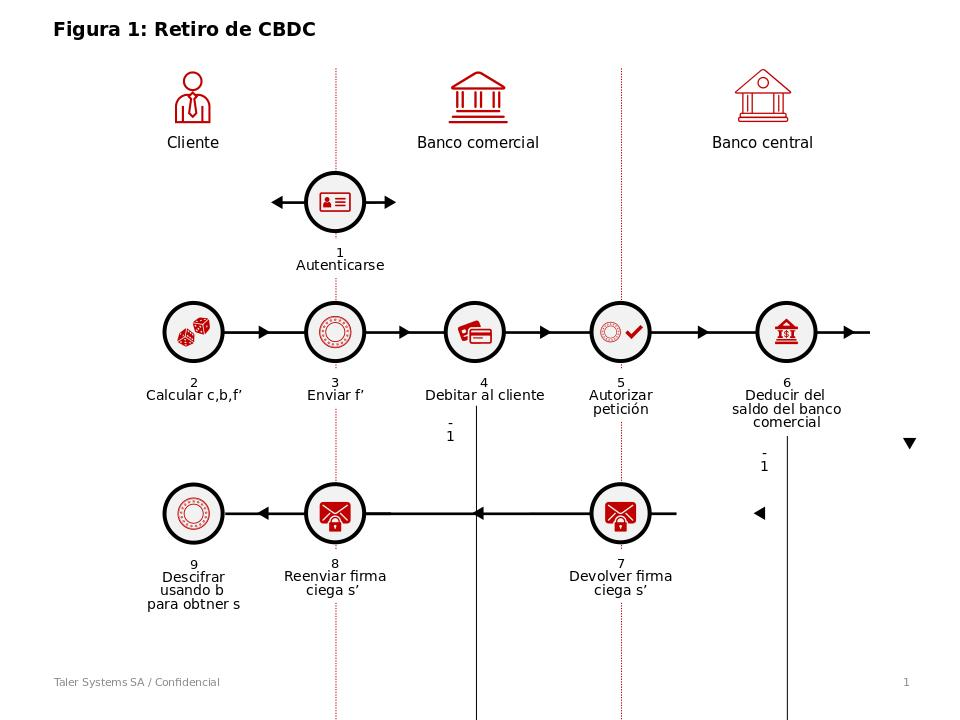
\includegraphics[width=\textwidth]{taler_figure_1_dora_SPANISH.jpg}

Un cliente (1) proporciona autenticación a su banco comercial usando la
autenticación respectiva del banco comercial y los procedimientos de
autorización. A continuación, el teléfono (u ordenador) del cliente
obtiene la clave de denominación $(e, n)$ provista por el banco central
para ese valor; calcula entonces (2) un par de claves para una moneda,
con la clave privada c y la clave pública $C$, y elige un factor de cegado
$b$. A la clave pública de la moneda se le aplica una función hash
($\to$ $f$) y es cegada ($\to$ $f'$). A continuación, (3) el teléfono
del cliente envía $f'$ junto con una autorización para retirar la
moneda y debitar de la cuenta del cliente en el banco comercial a través
de un canal seguro establecido. El banco comercial entonces (4) debita
la cantidad en la cuenta de depósito del cliente, (5) autoriza
digitalmente la petición con la propia firma digital de su sucursal
bancaria y reenvía la petición y la moneda cegada al banco central para
su firma. El banco central (6) deduce el valor de la moneda en la cuenta
del banco comercial, firma la moneda de forma ciega con la clave privada
del banco central para el valor respectivo, y (7) devuelve la firma
ciega $s'$ al banco comercial. (8) reenvía la firma ciega $s'$
a la billetera electrónica del cliente. Finalmente, el teléfono del
cliente (9) usa $b$ para descifrar la firma ($\to$ $f$) y almacena la
moneda recién acuñada $(c, s)$.

Cuando se gastan CBDC, el proceso es análogo a pagar al vendedor en
efectivo. Sin embargo, para asegurar el acuerdo, el vendedor debe
depositar las monedas. El procedimiento para gastar CBDC se indica en la
Figura 2.

Un cliente y un vendedor negocian un contrato comercial, y (1) el
cliente usa una moneda electrónica para firmar el contrato o factura de
venta con la clave privada $c$ de la moneda y transmite la firma al
vendedor. La firma de una moneda en un contrato con una moneda válida es
una instrucción del cliente para pagar al vendedor que es identificado
por la cuenta bancaria en el contrato. Los clientes pueden firmar
contratos con múltiples monedas en caso de que una sola moneda fuera
insuficiente para pagar la cantidad total. El vendedor (2) valida
entonces la firma de la moneda sobre el contrato y la firma s del banco
central sobre $f$ que corresponde a la $C$ de la moneda con las
respectivas claves públicas y reenvía la moneda firmada (junto con la
información de la cuenta del vendedor) al banco comercial del vendedor.
El banco comercial del vendedor (3) confirma que el vendedor es uno de
sus clientes y envía la moneda firmada al banco central. El banco
central (4) verifica las firmas y comprueba su base de datos para
asegurar que la moneda no haya sido previamente gastada. Si todo está en
orden, (5) el banco central añade la moneda a la lista de monedas
gastadas, acredita la cuenta del banco comercial en el banco central y
(6) envía la confirmación al banco comercial a tal efecto. A
continuación, (7) el banco comercial acredita la cuenta del vendedor e
(8) informa al vendedor. El vendedor (9) entrega el producto o servicio
al cliente. Todo el proceso dura solo unos pocos milisegundos.

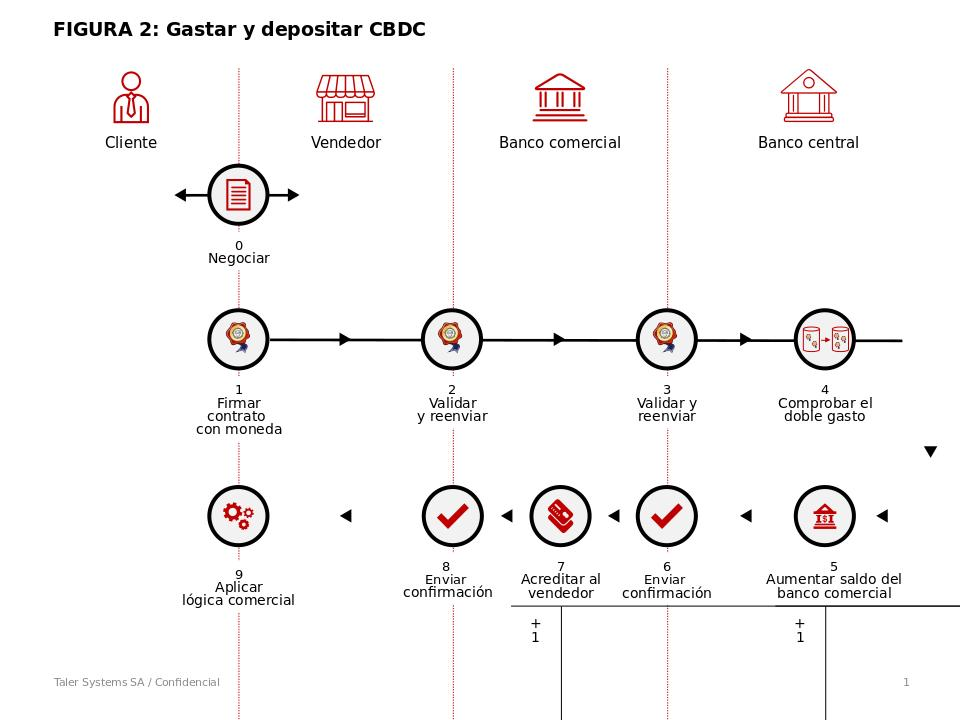
\includegraphics[width=\textwidth]{taler_figure_2_dora_SPANISH.jpg}.

\hypertarget{consideraciones-acerca-de-la-seguridad}{%
\subsection{Consideraciones acerca de la Seguridad}
\label{consideraciones-acerca-de-la-seguridad}}

Nuestra propuesta requiere que el banco central opere un servicio en
línea y una base de datos de alta disponibilidad. Debido a que los
usuarios pueden copiar las monedas electrónicas, solo los controles en
línea pueden prevenir eficientemente el doble gasto. Si bien existen
soluciones teóricas para identificar de manera retroactiva a usuarios
que se dediquen al doble gasto (véase Chaum et al. 1990), tales
soluciones crean un riesgo económico tanto para los usuarios como para
el banco central, debido al retraso en la identificación de
transacciones fraudulentas. La detección del doble gasto en línea
elimina este riesgo, pero a su vez implica que las transacciones serán
imposibles de realizar si la conexión con el banco central no estará
disponible.

El banco central también tendrá que proteger la confidencialidad de las
claves privadas que utiliza para firmar las monedas y otros mensajes del
protocolo. De manera que si las claves de las firmas del banco central
se vieran en algún momento comprometidas, como por ejemplo por una
computadora cuántica, un ataque físico en su centro de datos, o quizás
por algún nuevo algoritmo imprevisto, los usuarios puedan de forma
segura, y sin comprometer su privacidad, ser reembolsados con todas las
monedas que no han gastado. El banco central anunciaría la revocación de
clave mediante la API (Application Programming Interface), que sería
detectada por las billeteras e iniciarían el siguiente protocolo de
actualización: el usuario revela al banco central la clave pública
$C$ de la moneda, la firma $s$ del banco central, y el factor
ciego $b$, posibilitando así que el banco central verifique el
retiro legítimo del usuario y devuelva el valor de la moneda no gastada.
Para detectar un posible compromiso de esta clave, el banco central
puede monitorear la base de datos en busca de casos de depósitos que
superen los retiros.

\hypertarget{escalabilidad-y-costes}{%
\subsection{Escalabilidad y Costes}\label{escalabilidad-y-costes}}

El esquema que proponemos sería tan eficiente y rentable como los
modernos sistemas RTGS que utilizan actualmente los bancos centrales.

La escalabilidad se refiere al costo de aumentar la capacidad de
procesamiento para que se pueda procesar un número cada vez mayor de
transacciones en un tiempo adecuado para la finalidad. El costo global
del sistema puede ser bajo, ya que la CBDC que se propone aquí se basa
en software solamente. Las monedas gastadas deben guardarse hasta que
caduque el par de claves de denominación que se usó para firmar las
monedas; por ejemplo, mediante un calendario anual renovable, que
mantiene limitado el tamaño de la base de datos. La cantidad de potencia
de procesamiento adicional y ancho de banda necesarios aumenta en la
misma cantidad por cada transacción, gasto o depósito adicional, porque
las transacciones son esencialmente independientes una de la otra. Esta
potencia adicional se logra simplemente añadiendo más hardware,
comúnmente llamado partición o fragmentación. Con el llamado hash
consistente, las adiciones de hardware no tienen por qué ser
disruptivas. Se puede utilizar cualquier tecnología de base de datos
subyacente.

Más concretamente, la lógica del front-end en el banco central solo
tiene que realizar unas cuantas operaciones de firma, y un único
procesador puede hacer miles de operaciones por segundo (véase Bernstein
y Lange 2020). Si un solo sistema es insuficiente, es fácil desplegar
servidores front-end adicionales y solicitar a los varios bancos
comerciales que balanceen sus peticiones en la granja de servidores o
que utilicen un balanceador de carga para distribuir las peticiones
dentro de la infraestructura del banco central.

Los servidores front-end deben comunicarse con una base de datos para
hacer transacciones y prevenir el doble gasto. Un solo servidor moderno
para la base de datos debería ser suficiente para manejar de manera
fiable decenas de miles de estas operaciones por segundo. Las
operaciones se reparten fácilmente entre varios servidores de bases de
datos simplemente asignando a cada servidor un rango de valores de los
que es responsable. Este diseño asegura que las transacciones
individuales nunca crucen fragmentos. Así, se espera que también los
sistemas de back-end escalen linealmente con los recursos
computacionales disponibles, de nuevo partiendo de una línea de base
alta para un solo sistema.

Los front-end también deben comunicarse con los back-end mediante una
interconexión. Las interconexiones puede soportar grandes cantidades de
transacciones por segundo. El tamaño de una transacción individual suele
ser de 1-10 kilobytes aproximadamente. Asi, las interconexiones de un
centro de datos moderno, con velocidades de conmutación de 400 Gbit/s,
pueden soportar millones de transacciones por segundo.

En fin, el costo total del sistema es bajo. Es probable que el
almacenamiento seguro de 1 a 10 kilobytes por transacción durante muchos
años sea el costo predominante del sistema. Utilizando los precios de
Amazon Web Services, experimentamos con un prototipo anterior de GNU
Taler y descubrimos que el costo del sistema (almacenamiento, ancho de
banda y computación) a escala estaría por debajo de USD 0,0001 por
transacción (para obtener detalles sobre los datos, consulte Dold 2019).

\hypertarget{consideraciones-normativas-y-poluxedticas}{%
\section{Consideraciones normativas y políticas}\label{5.-consideraciones-normativas-y-poluxedticas}}

En el esquema propuesto, los bancos centrales no conocen la identidad de
los consumidores o comerciantes ni los montos totales de las
transacciones. Los bancos centrales solo ven cuándo se lanzan las
monedas electrónicas y cuándo se canjean. Los bancos comerciales siguen
proporcionando autenticación crucial de clientes y comerciantes y, en
particular, siguen siendo los guardianes de la información del KYC. Los
bancos comerciales observan cuándo los comerciantes reciben fondos y
pueden limitar la cantidad de CBDC por transacción que un comerciante
individual puede recibir, si así se requiere.

Además, las transacciones están asociadas con los contratos pertinentes
de los clientes. La transparencia de ingresos que se obtiene permite que
el sistema cumpla con los requisitos del AML y CFT. Si se detectan
patrones inusuales de ingresos comerciales, el banco comercial, las
autoridades fiscales o las fuerzas del orden pueden obtener e
inspeccionar los contratos comerciales subyacentes a los pagos para
determinar si la actividad sospechosa es ilegal. La transparencia de los
ingresos que se obtiene es también una fuerte medida contra la evasión
fiscal porque los comerciantes no pueden declarar menos ingresos o
evadir los impuestos sobre las ventas. En general, el sistema implementa
privacidad por diseño y privacidad por omisión (como lo exige, por
ejemplo, el Reglamento General de Protección de Datos de la Unión
Europea). Los comerciantes no infieren inherentemente la identidad de
sus clientes, los bancos solo tienen la información necesaria sobre las
actividades de sus propios clientes y los bancos centrales están
felizmente divorciados del conocimiento detallado de las actividades de
los ciudadanos.

Por razones reglamentarias, en algunos países existen límites para los
retiros y pagos en efectivo. Dichas restricciones también podrían
implementarse para la CBDC en el diseño propuesto. Por ejemplo, se
podría limitar la cantidad que los consumidores puedan retirar por día,
o limitar la cantidad total de CBDC que los bancos comerciales puedan
convertir.

Un problema potencial de estabilidad financiera que a menudo se plantea
con las CBDC al por menor es la desintermediación del sector bancario.
En particular, la venta de CBDC al por menor podría facilitar el
acaparamiento de grandes cantidades de dinero del banco central. Esto
podría afectar negativamente a la financiación de depósitos de los
bancos porque el público tendría menos dinero en forma de depósitos
bancarios. Para los países cuyas monedas sirven como monedas de refugio
seguro, podría conducir a un aumento de las entradas de capital durante
períodos de riesgo global, lo que resultaría en presiones adicionales en
la apreciación del tipo de cambio.

Si bien esto podría representar una preocupación seria en el caso de una
CBDC basada en cuentas, la preocupación sería menor con una CBDC basada
en tokens. En primer lugar, acumular una CBDC basada en tokens conlleva
riesgos de robo o pérdida similares a los de acumular efectivo. Tener
unos cientos de dólares en un teléfono inteligente es probablemente un
riesgo aceptable para muchos, pero tener una cantidad muy grande es
probablemente un riesgo menos aceptable. Por tanto, no esperaríamos un
acaparamiento significativamente mayor que en el caso del efectivo
físico.

Sin embargo, si el acaparamiento o la conversión masiva a CBDC de dinero
proveniente de depósitos bancarios se convirtieran en un problema, los
bancos centrales tendrían varias opciones. Como se señaló, en el diseño
propuesto los bancos centrales configuran una fecha de vencimiento para
todas las claves de firma, lo que implica que en una fecha establecida
las monedas firmadas con esas claves dejan de ser válidas. Cuando las
claves de denominación caducan y los clientes tienen que cambiar monedas
firmadas con claves de denominación antiguas por monedas nuevas, el
regulador podría fácilmente imponer un límite de conversión por cliente
para hacer cumplir un límite estricto a la cantidad de CBDC que
cualquier individuo puede acumular. Además, los bancos centrales podrían
cobrar una tarifa si fuera necesario. Una tarifa de actualización de
este tipo, cuando las monedas están programadas para caducar, implicaría
de hecho tasas de interés negativas en la CBDC, y haría que la CBDC
resultara menos atractiva como depósito de valor, tal como sugiere
Bindseil (2020). De hecho, sería la implementación directa de la idea de
Silvio Gesell de aplicar un ``impuesto de posesión'' sobre la moneda, al
que hace célebremente referencia Keynes (1936), y reviven Goodfriend
(2000), Buiter y Panigirtzoglou (2003) y Agarwal y Kimball (2019).

En cuanto a las posibles implicaciones para las políticas monetarias, no
anticipamos efectos materiales porque nuestra CBDC está diseñada para
replicar el dinero en efectivo en lugar de los depósitos bancarios. La
emisión, retiro y depósito de nuestra CBCD corresponden exactamente a la
emisión, retiro y depósito de billetes. Es posible que una CBDC al por
menor tenga un ritmo de circulación diferente a la del efectivo físico,
pero esto no sería un problema material para las políticas monetarias.

\hypertarget{trabajos-relacionados}{%
\section{Trabajos relacionados}\label{6.-trabajos-relacionados}}

Como se señaló anteriormente, la CBDC propuesta en el presente documento
se basa en eCash y GNU Taler.\footnote{La implementación de eCash por la
compañía DigiCash en los años noventa está documentada en
\url{https://www.chaum.com/ecash}.} A
partir de la propuesta original de Chaum para el efectivo electrónico,
la investigación se ha centrado en tres cuestiones principales. Primero,
en la propuesta original de Chaum las monedas tenían un valor fijo y
solo podían gastarse en su totalidad. Pagar grandes cantidades con
monedas denominadas en centavos sería ineficiente, por lo que Okamoto
(1995), Camenisch (2005), Canard y Gouget (2007) y Dold (2019) idearon
formas de abordar este problema. Estas soluciones involucran protocolos
para dar cambio o para posibilitar la divisibilidad de las monedas.

Una segunda cuestión es que las transacciones a veces fallan debido a
caídas de la red, por ejemplo. En este caso, el sistema debe permitir
que los fondos permanezcan con el consumidor sin impacto negativo sobre
privacidad. Camenisch et al. (2007) y Dold (2019) abordan este tema en
su propuesta de dinero electrónico respaldado. Varias de las soluciones
anteriores violan las garantías de privacidad para los clientes que
utilizan estas funciones, y todas, excepto Taler, violan el requisito de
transparencia de ingresos.

La tercera cuestión importante, a menudo desatendida, es conservar la
transparencia de los ingresos y, por lo tanto, el cumplimiento del AML y
KYC. Fuchsbauer y col. (2009) diseñaron deliberadamente un sistema que
posibilita la desintermediación para proporcionar una semántica más
similar al efectivo. Sin embargo, la desintermediación ilimitada
generalmente no concuerda con las regulaciones del AML y KYC, ya que no
permite lograr ningún nivel de responsabilidad. Un ejemplo de tal diseño
es ZCash, un libro mayor distribuido que oculta a la red la información
sobre el pagador, el beneficiario y el monto de la transacción, siendo
por lo tanto el sistema de pago perfecto para la delincuencia en línea.
Solo Taler ofrece tanto la privacidad constante del cliente como la
transparencia de los ingresos, al mismo tiempo que proporciona un cambio
eficiente, intercambios atómicos (consulte Camenisch 2007) y la
capacidad de restaurar billeteras desde una copia de seguridad.

Con respecto a los sistemas de pago para las CBDC, Danezis y Meiklejohn
(2016) diseñaron un libro mayor escalable con RSCoin. Básicamente es un
sistema RTGS que es protegido utilizando la misma criptografía que se
usa en Bitcoin. Al igual que Taler, el diseño utiliza la fragmentación
de la base de datos para lograr una escalabilidad lineal. Sin embargo,
el diseño de Danezis y Meiklejohn no tiene ninguna disposición para la
privacidad y carece de consideraciones sobre cómo integrar prácticamente
el diseño con los sistemas y procesos bancarios existentes.

La EUROchain del Banco Central Europeo (véase ECB 2019) es otro
prototipo para CBDC con libro mayor distribuido. Similar a la
arquitectura propuesta en el presente documento, la EUROchain utiliza
una arquitectura de dos niveles donde los bancos comerciales actúan como
intermediarios. Una diferencia crucial es la manera en que los sistemas
intentan combinar la privacidad y el cumplimiento del AML. En nuestro
diseño, los reguladores podrían imponer un límite a la cantidad de
efectivo electrónico que el titular de una cuenta bancaria puede retirar
durante un cierto tiempo, mientras que la EUROchain emite un número
limitado de "vales de anonimato" que conceden al receptor un número
limitado de transacciones sin verificación del AML. Como estos vales
parecen no tener ninguna relación con ningún token de valor, no queda
claro de qué manera el diseño evitaría la aparición de un mercado negro
de ``vales de anonimato''. Además, la noción de anonimato de la
EUROchain es muy diferente, ya que sus "vales de anonimato" simplemente
eliminan ciertas verificaciones del AML, al mismo tiempo que preservan
la capacidad de los bancos comerciales de ver cómo los consumidores
gastan el efectivo electrónico. Mientras que los pagadores usuarios de
Taler interactúan directamente con los comerciantes para gastar su
efectivo electrónico, el sistema EUROchain requiere que los pagadores
instruyan a sus bancos comerciales para que accedan a su CBDC. Por lo
tanto, la EUROchain no emite tokens de valor directamente a los
consumidores y, en cambio, depende de que los consumidores se
autentiquen ellos mismos en sus bancos comerciales para acceder a la
CBDC que el banco central mantiene efectivamente en custodia. Por lo
tanto, no está claro qué ventajas de privacidad, rendimiento o seguridad
tiene la EUROchain sobre el dinero existente en depósito.

\hypertarget{conclusiuxf3n}{%
\section{Conclusión}
\label{7.-conclusiuxf3n}}

Con la aparición de Bitcoin y monedas digitales recientemente propuestas
por grandes empresas tecnológicas como Diem (antes Libra), los bancos
centrales se enfrentan a una competencia cada vez mayor de actores que
ofrecen su propia alternativa digital al efectivo físico. Las decisiones
de los bancos centrales sobre la emisión o no de una CBDC dependen de
cómo evalúen los beneficios y los riesgos de una CBDC. Estos beneficios
y riesgos, así como las circunstancias jurisdiccionales específicas que
definen el alcance de las CBDC al por menor, probablemente difieran de
un país a otro.

Si un banco central decide emitir una CBDC al por menor, proponemos una
CBDC basada en tokens que combina la privacidad de las transacciones con
el cumplimiento del KYC, AML y CFT. Dicha CBDC no competiría con los
depósitos de los bancos comerciales, sino que reproduciría el efectivo
físico, lo que limitaría los riesgos de estabilidad financiera y
políticas monetarias.

Hemos demostrado que el esquema propuesto aquí sería tan eficiente y
rentable como los sistemas RTGS modernos operados por los bancos
centrales. Los pagos electrónicos con nuestra CBDC solo necesitarían una
simple base de datos para las transacciones y cantidades minúsculas de
ancho de banda. La eficiencia y la rentabilidad, junto con la facilidad
de uso mejorada para el consumidor provocada por el cambio de la
autenticación a la autorización, hacen que este esquema sea
probablemente el primero en respaldar el objetivo largamente previsto de
los micropagos en línea. Además, el uso de monedas para firmar
criptográficamente contratos electrónicos permitiría el uso de contratos
inteligentes. Esto también podría conducir a la aparición de
aplicaciones completamente nuevas para los sistemas de pago. Aunque
nuestro sistema no se basa en la DLT, podría integrarse fácilmente con
dichas tecnologías si así lo requirieran las infraestructuras del
mercado financiero en el futuro.

Igualmente importante, sin embargo, es que una CBDC al por menor debe
preservar el efectivo como un bien común respetuoso de la privacidad
bajo el control individual de los ciudadanos. Esto se puede lograr con
el esquema propuesto en este documento, y los bancos centrales pueden
evitar perturbaciones significativas en sus políticas monetarias y
estabilidad financiera cosechando al mismo tiempo los beneficios de la
digitalización.


\newpage
REFERENCIAS

\begin{itemize}
\item Adrian, Tobias and Tommaso Mancini-Griffoli. 2019. ``The Rise of Digital
Money.'' IMF Fintech Note 19/01.
\end{itemize}

\begin{itemize}
\item Agarwal, Ruchir and Miles S. Kimball. 2019. ``Enabling Deep Negative
Rates to Fight Recessions: A Guide.'' IMF Working Paper 19/84.
\end{itemize}

\begin{itemize}
\item Agur, Itai, Anil Ari and Giovanni Dell'Ariccia. 2019. ``Designing
Central Bank Digital Currencies.'' IMF Working Paper 19/252.
\end{itemize}

\begin{itemize}
\item Allen, Sarah, Srđjan Čapkun, Ittay Eyal, Giulia Fanti, Bryan A. Ford,
James Grimmelmann, Ari Juels, Kari Kostiainen, Sarah Meiklejohn, Andrew
Miller, Eswar Prasad, Karl Wüst, and Fan Zhang. 2020. ``Design Choices
for Central Bank Digital Currency: Policy and Technical
Considerations.'' NBER Working Paper No. 27634.
\end{itemize}

\begin{itemize}
\item Alves, Tiago and Don Felton. 2004. ``TrustZone: Integrated hardware and
software security.'' ARM IQ, Vol. 3, No. 4, pp. 18--24.
\end{itemize}

\begin{itemize}
\item Auer, Raphael and Rainer Böhme. 2020. ``The technology of retail central
bank digital currency\emph{.''} BIS Quarterly Review, March 2020, pp.
85--96.
\end{itemize}

\begin{itemize}
\item Auer, Raphael, Giulio Cornelli and Jon Frost. 2020. ``Taking stock:
ongoing retail CBDC projects.'' BIS Quarterly Review, March 2020, pp.
97--98.
\end{itemize}

\begin{itemize}
\item Bank for International Settlements. 2018. ``Central Bank Digital
Currencies.'' Joint Report of the Committee on Payments and Market
Infrastructures and Markets Committee.
\end{itemize}

\begin{itemize}
\item Bank of England. 2020. ``Central Bank Digital Currency: Opportunities,
Challenges and Design.'' Discussion Paper. March.
\end{itemize}

\begin{itemize}
\item Baiocchi, Giovanni and Walter Distaso. 2003. ``GRETL: Econometric
Software for the GNU Generation.'' Journal of Applied Econometrics, Vol.
18, pp. 105-110.
\end{itemize}

\begin{itemize}
\item Bech, Morten and Rodney Garratt. 2017. ``Central bank
cryptocurrencies.'' BIS Quarterly Review, September, pp. 55--70.
\end{itemize}

\begin{itemize}
\item Berentsen, Aleksander and Fabian Schär. 2018. ``The Case for Central
Bank Electronic Money and the Non-case for Central Bank
Cryptocurrencies.'' Federal Reserve Bank of St. Louis Review, Vol. 100,
No. 2, pp. 97--106.
\end{itemize}

\begin{itemize}
\item Bernstein, Daniel J. and Tanja Lange. 2020. ``eBACS: ECRYPT Benchmarking
of Cryptographic Systems.'' https://bench.cr.yp.to, accessed 17 March
2020.
\end{itemize}

\begin{itemize}
\item Bernstein, Daniel J., Niels Duif, Tanja Lange, Peter Schwabe, and Bo-Yin
Yang. 2012. ``High-speed high-security signatures.'' Journal of
Cryptographic Engineering, Vol. 2, pp. 77--89.
\end{itemize}

\begin{itemize}
\item Bindseil, Ulrich. 2020. ``Tiered CBDC and the financial system.'' ECB
Working Paper 2351 January.
\end{itemize}

\begin{itemize}
\item Boar, Codruta, Henry Holden and Amber Wadsworth. 2020. ``Impending
arrival - a sequel to the survey on central bank digital currency.'' BIS
Papers, No. 107.
\end{itemize}

\begin{itemize}
\item Boneh, Dan. 1999. ``Twenty Years of Attacks on the RSA Cryptosystem.''
Notices of the AMS, Vol. 42, No. 2, pp. 202--213.
\end{itemize}

\begin{itemize}
\item Bordo, Michael D. and Andrew T. Levin. 2017. ``Central bank digital
currency and the future of monetary policy.'' NBER Working Papers No.
23711.
\end{itemize}

\begin{itemize}
\item Brunnermeier, Markus and Dirk Niepelt. 2019. ``On the Equivalence of
Private and Public Money.'' Journal of Monetary Economics, Vol. 106, pp.
27--41.
\end{itemize}

\begin{itemize}
\item Buiter, Willem H. and Nikolaos Panigirtzoglou. 2003. ``Overcoming the
Zero Bound on Nominal Interest Rates with Negative Interest on Currency:
Gesell's Solution.'' The Economic Journal, Vol. 113, No. 490, pp.
723--746.
\end{itemize}

\begin{itemize}
\item Bullmann, Dirk, Jonas Klemm and Andrea Pinna. 2019. ``In search for
stability in crypto-assets: are stablecoins the solution?'' ECB
Occasional Paper Series No. 230.
\end{itemize}

\begin{itemize}
\item Camenisch, J., Aanna Lysyanskaya, and Mira Meyerovich. 2007. ``Endorsed
E-Cash.'' In: 2007 IEEE Symposium on Security and Privacy (SP '07). May:
pp.101--115.
\end{itemize}

\begin{itemize}
\item Camenisch, Jan, Susan Hohenberger, and Anna Lysyanskaya. 2005. ``Compact
E-Cash.'' In: Advances in Cryptology -- EUROCRYPT 2005: 24th Annual
International Conference on the Theory and Applications of Cryptographic
Techniques, Aarhus, Denmark, May 22-26, 2005. Proceedings. Ed. by Ronald
Cramer. Berlin, Heidelberg: Springer.
\end{itemize}

\begin{itemize}
\item Canard, Sébastien and Aline Gouget. 2007. ``Divisible e-cash systems can
be truly anonymous.'' In: Annual International Conference on the Theory
and Applications of Cryptographic Techniques. pp. 482--97.
\end{itemize}

\begin{itemize}
\item CCC. 2017. ``Chaos Computer Club hacks e-motor charging stations.''
34c3.
\end{itemize}

\begin{itemize}
\item Chapman, James, Rodney Garratt, Scott Hendry, Andrew McCormack and Wade
McMahon. 2017. Project Jasper: Are Distributed Wholesale Payment Systems
Feasible Yet? Bank of Canada, Financial System Review, June, pp. 59--69.
\end{itemize}

\begin{itemize}
\item Chaum, David. 1983. ``Blind signatures for untraceable payments.''
Advances in Cryptology: Proceedings of Crypto `82, Vol. 82, No. 3, pp.
199--203.
\end{itemize}

\begin{itemize}
\item Chaum, David, Amos Fiat, and Moni Naor. 1990. ``Untraceable electronic
cash.'' Advances in Cryptology: Proceedings of CRYPTO '88, pp. 319--327.
\end{itemize}

\begin{itemize}
\item Danezis, George and Sarah Meiklejohn. 2016. ``Centrally Banked
Cryptocurrencies.'' In: 23nd Annual Network and Distributed System
Security Symposium, NDSS2016, San Diego, California, USA, February
21--24. The Internet Society.
\end{itemize}

\begin{itemize}
\item Diffie, Whitfield and Martin Hellmann. 1976. ``New Directions in
Cryptography''. IEEE Trans. on Inf. Theory, IT-22, pp. 644--654.
\end{itemize}

\begin{itemize}
\item Dold, Florian. 2019. The GNU Taler System: Practical and Provably Secure
Electronic Payments. PhD Thesis, University of Rennes 1.
\end{itemize}

\begin{itemize}
\item European Central Bank. 2019. ``Exploring anonymity in central bank
digital currencies.'' In: In Focus, Issue No. 4, December.
\end{itemize}

\begin{itemize}
\item Fuchsbauer, Georg, David Pointcheval, and Damien Vergnaud. 2009.
``Transferable constant-size fair e-cash.'' In: International Conference
on Cryptology and Network Security. Springer. pp. 226--47.
\end{itemize}

\begin{itemize}
\item Garcia, Flavio, Gerhard de Koning Gans, Ruben Muijrers, Peter van
Rossum, Roel Verdult, Ronny Wichers Schreur and Bart Jacobs. 2008.
``Dismantling MIFARE Classic.'' European Symposium on Research in
Computer Security.
\end{itemize}

\begin{itemize}
\item Garratt, Rod, Michael Lee, Brendan Malone, and Antoine Martin. 2020.
``Token- or Account-Based? A Digital Currency Can Be Both.'' Liberty
Street Economics, Federal Reserve Bank of New York, August 12, 2020.
\end{itemize}

\begin{itemize}
\item Goodfriend, Marvin. 2000. ``Overcoming the Zero Bound on Interest Rate
Policy.'' Journal of Money, Credit, and Banking, Vol. 32, No. 4,
1007--35.
\end{itemize}

\begin{itemize}
\item Johnston, Casey. 2010. ``PS3 hacked through poor cryptography
implementation.'' Ars Technica, December 30.
\end{itemize}

\begin{itemize}
\item Jordan, Thomas J. 2019. ``Currencies, money and digital tokens.'' Speech
given at the 30th anniversary of the WWZ and VBÖ, University of Basel,
September. Available at:
www.snb.ch/en/mmr/speeches/id/ref\_20190905\_tjn/source/ref\_20190905\_tjn.en.pdf
\end{itemize}

\begin{itemize}
\item Kahn, Charles M. and William Roberds. 2009. ``Why Pay? An Introduction
to Payments Economics.'' Journal of Financial Intermediation, No. 18,
pp. 1--23.
\end{itemize}

\begin{itemize}
\item Kahn, Charles M., James McAndrews, and William Roberds. 2005. ``Money is
Privacy.'' International Economic Review, Vol. 46, No. 2, pp. 377--399.
\end{itemize}

\begin{itemize}
\item Kasper, Timo, Michael Silbermann and Christof Paar. 2010. ``All you can
eat or breaking a real-world contactless payment system.'' Financial
Cryptography and Data Security, Lecture Notes in Computer Science, Vol.
6052, pp. 343--50.
\end{itemize}

\begin{itemize}
\item Katzenbeisser, Stefan, Ünal Kocabaş, Vladimir Rožić, Ahmad-Reza Sadeghi,
Ingrid Verbauwhede and Christian Wachsmann. 2012. ``PUFs: Myth, Fact or
Busted? A Security Evaluation of Physically Unclonable Functions (PUFs)
Cast in Silicon.'' Cryptographic Hardware and Embedded Systems -- CHES
2012. Lecture Notes in Computer Science, Vol. 7428, pp. 283--301.
\end{itemize}

\begin{itemize}
\item Keynes, John Maynard. 1936. The General Theory of Employment, Interest
and Money. London: Macmillan.
\end{itemize}

\begin{itemize}
\item Kiff, John, Jihad Alwazir, Sonja Davidovic, Aquiles Farias, Ashraf Khan,
Tanai Khiaonarong, Majid Malaika, Hunter Monroe, Nobu Sugimoto, Hervé
Tourpe, and Peter Zhou. 2020. A Survey of Research on Retail Central
Bank Digital Currency. IMF Working Paper 20/104.
\end{itemize}

\begin{itemize}
\item Kumhof, Michael and Clare Noone. 2018. ``Central bank digital currencies
- design principles and balance sheet implications.'' Bank of England,
Staff Working Paper No. 725.
\end{itemize}

\begin{itemize}
\item Lapid, Ben, and Avishai Wool. 2018. ``Cache-Attacks on the ARM TrustZone
Implementations of AES-256 and AES-256-GCM via GPU-Based Analysis.''
International Conference on Selected Areas in Cryptography. Lecture
Notes in Computer Science, Vol. 11349.
\end{itemize}

\begin{itemize}
\item Lerner, Josh and Jean Tirole. 2005. ``The Scope of Open Source
Licensing.'' Journal of Law, Economics \& Organization, Vol. 21, pp.
20-56.
\end{itemize}

\begin{itemize}
\item Libra Association. 2020. Libra White Paper v2.0.
\href{https://libra.org/en-US/white-paper/}{{https://libra.org/en-US/white-paper/}}
\end{itemize}

\begin{itemize}
\item Lim, Chae Hoon and Phil Joong Lee. 1997. ``A key recovery attack on
discrete log-based schemes using a prime order subgroup.'' CRYPTO 1997.
Lecture Notes in Computer Science, vol 1294.
\end{itemize}

\begin{itemize}
\item Lyons, Richard K. and Ganesh Viswanath-Natraj. 2020. ``What Keeps
Stablecoins Stable?'' NBER Working Paper No. 27136, May.
\end{itemize}

\begin{itemize}
\item Mancini-Griffoli, Tommaso, Maria Soledad Martinez Peria, Itai Agur, Anil
Ari, John Kiff, Adina Popescu, and Celine Rochon. 2018. ``Casting Light
on Central Bank Digital Currency.'' IMF Staff Discussion Notes 18/08,
International Monetary Fund.
\end{itemize}

\begin{itemize}
\item Nakamoto, Satoshi. 2008. Bitcoin: A Peer-to-Peer Electronic Cash System.
\href{https://www.bitcoin.com/bitcoin.pdf}{{https://www.bitcoin.com/bitcoin.pdf}}
\end{itemize}

\begin{itemize}
\item Narayanan, Arvind, Joseph Bonneau, Edward Felten, Andrew Miller, Steven
Goldfeder. 2016. Bitcoin and Cryptocurrency Technologies: A
Comprehensive Introduction. Princeton: Princeton University Press.
\end{itemize}

\begin{itemize}
\item Niepelt, Dirk. 2020. Digital money and central bank digital currency: An
executive summary for policymakers. VOX/CEPR.
\href{https://voxeu.org/article/digital-money-and-central-bank-digital-currency-executive-summary}{{https://voxeu.org/article/digital-money-and-central-bank-digital-currency-executive-summary}}.
\end{itemize}

\begin{itemize}
\item Okamoto, Tatsuaki. 1995. ``An Efficient Divisible Electronic Cash
Scheme.'' Advances in Cryptology --- CRYPT0'95: 15th Annual
International Cryptology Conference Santa Barbara, California, USA,
August 27--31, 1995 Proceedings. Ed. by Don Coppersmith. Berlin,
Heidelberg: Springer, pp. 438--451.
\end{itemize}

\begin{itemize}
\item Pinto, S. and N. Santos. 2019. ``Demystifying Arm TrustZone: A
Comprehensive Survey.'' ACM Computing Surveys, Article No. 130, January.
\end{itemize}

\begin{itemize}
\item Rivest, Ronald L., Adi Shamir, and Leonard Adleman. 1978. ``A Method for
Obtaining Digital Signatures and Public Key Cryptosystems''. Comm. ACM,
Vol 21, No 2.
\end{itemize}

\begin{itemize}
\item Solove, Daniel J. 2011. Nothing to Hide: The false tradeoff between
privacy and security. New Haven \& London: Yale University Press.
\end{itemize}

\begin{itemize}
\item Soukup, Michael and Bruno Muff. 2007. ``Die Postcard lässt sich
fälschen.'' Sonntagszeitung, April 22.
\end{itemize}

\begin{itemize}
\item Stallman, Richard. 1985. The GNU manifesto. Dr. Dobb's Journal of
Software Tools 10(3), pp. 30--35.
\end{itemize}

\begin{itemize}
\item Sveriges Riksbank. 2020. The Riksbank's e-krona project. February.
https://www.riksbank.se/globalassets/media/rapporter/e-krona/2019/the-riksbanks-e-krona-pilot.pdf
\end{itemize}

\begin{itemize}
\item Wojtczuk, Rafal and Joanna Rutkowska. 2009. ``Attacking Intel Trusted
Execution Technology.'' BlackHat-DC 2009.
\end{itemize}

\begin{itemize}
\item Yalta, A.Talha, and A. Yasemin Yalta. 2010. ``Should Economists Use Open
Source Software for Doing Research?'' Computational Economics, Vol. 35,
pp. 371--94.
\end{itemize}

\begin{itemize}
\item Yalta, A. Talha, and Riccardo Lucchetti. 2008. ``The GNU/Linux Platform
and Freedom Respecting Software for Economists.'' Journal of Applied
Econometrics, Vol. 23, pp. 279-86.
\end{itemize}

\bibliographystyle{plain}
\bibliography{cbdc,rfc}

\end{document}
